\section{Interaction Design Process}
Interaction design can be briefly defined as "designing interactive products to support people in their everyday working lives" \cite{Sharp2011}. To develop a useful product an understanding of what is needed must be established before and during the development process. This brings new challenges and questions, such as if users understand what are they expecting from a specific product; and, of course, correctly establishing who the users are beforehand. Interaction design process is a strong user-centered methodology, that, correctly carried out will output a product that reflects the real user voice and needs. An user must be understood as the persons that will use the product for the intended goals. The stakeholders are the persons that are involved in the development process influencing the system requirements. For the purposes of this project, the users are the general public who are concerned with air quality and how it can have an impact on their health status. The stakeholders are the secondary agents who have provided an opinion on the capabilities of the system, in this case are my project supervisor and other researchers in the field that can give formative feedback.

As described in Figure \ref{fig:interaction_design}, the interaction design process is carried out with four activities: \begin{itemize}
  \item Identify user needs and establishing requirements
  \item Develop alternative designs
  \item Build interactive versions
  \item Evaluation with users
\end{itemize}

\begin{figure}[h]
  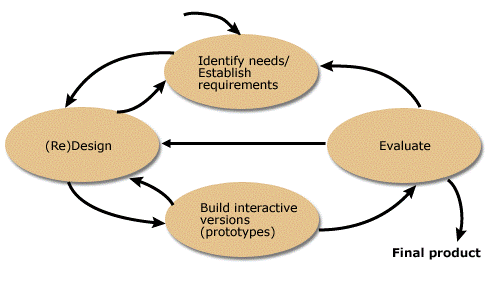
\includegraphics[scale=.8]{images/interatcion-design.png}
  \caption[Interaction design process]{Interaction design process \cite{Sharp2011}}
  \label{fig:interaction_design}
\end{figure}

Identifying needs and establishing requirements is the first and most crucial activity of the process. Its objective is to learn and understand the user needs and communicate them to the developer. According to the chaos report \cite{Group1994}, requirements account for more than the 30\% of the project failure factors, they include lack  of user input, incomplete requirements and specifications, or changes in requirements and specifications. Also its interdisciplinary nature, and contradictions between stakeholders add complexity to this part of the process. To guide it in a more accurate and disciplined manner, it is useful to combine different techniques and methodologies, such as questionnaires, interviews, introspection and brainstorming \cite{Coulin2005}. The selected methods were questionnaires and interviews. Interviews allowed to establish a casual conversation with few potential application users, whereas questionnaires allowed to get different points of views of many potential users of the application. 

A support tool for developing alternative designs is the prototype. It is a physical, or digital outline of a screen or task supported by the product. It allows for different purposes: first, as support for the creative process, allowing the designer to print how is the interface expected to look like and how it will support the intended use cases. Second, as a communication tool for the stakeholders, supporting the flow of ideas between the designer and the people involved in the development. And third, as a testing tool, allowing the designer to get measurable feedback of the capabilities of the product. Prototypes were designed and evaluated in different iterations among the project.